\subsection{Series Tests}

% **Role:** convergence of functions and analytic approximation.
%
% Series, absolute/conditional convergence, comparison tests, ratio/root tests, rearrangements, products, double sums.


Series are sequences of partial sums. Comparison, condensation, root and ratio tests, rearrangements, products, and double sums all refine that viewpoint.

\begin{definition} \label{def:series-and-partial-sums} \hlt{Series and Partial Sums}\\
Let $n_0\in\N_0$ and $(a_n)_{n\geq n_0}\subseteq\C$. Summation indices are bound variables and may be renamed within unchanged scope.
\begin{enumerate}[label=(\roman*)]
\setlength{\itemsep}{0pt}
\item For integers $n_0\leq p\leq q$, $\sum\limits_{n=p}^{q}a_n\defeq a_p+a_{p+1}+\cdots+a_q$.
\item The \hlt{series} $\sum\limits_{n=n_0}^{\infty}a_n$ is the \hlt{partial-sum sequence} $(s_N)_{N\geq n_0}$, where $s_N\defeq\sum\limits_{n=n_0}^{N}a_n$.
\item The series \hlt{converges to} $s$, written $\sum\limits_{n=n_0}^{\infty}a_n=s$, iff $s_N\to s$; otherwise it \hlt{diverges}.
\end{enumerate}
\hlt{Key Insight}: A series is a sequence first; its sum is a limit when that limit exists.
\end{definition}

\begin{definition} \label{def:absolute-and-nonabsolute-convergence} \hlt{Absolute and Nonabsolute Convergence}\\
Let $n_0\in\N_0$ and $(a_n)_{n\geq n_0}\subseteq\C$.
\begin{enumerate}[label=(\roman*)]
\setlength{\itemsep}{0pt}
\item The series $\sum\limits_{n=n_0}^{\infty}a_n$ \hlt{converges absolutely} iff $\sum\limits_{n=n_0}^{\infty}\abs{a_n}$ converges.
\item The series $\sum\limits_{n=n_0}^{\infty}a_n$ \hlt{converges nonabsolutely} iff it converges and $\sum\limits_{n=n_0}^{\infty}\abs{a_n}$ diverges.
\end{enumerate}
\end{definition}

\begin{theorem} \label{thm:series-cauchy-criterion} \hlt{Cauchy Criterion for Series}\\
Let $n_0\in\N_0$, $(a_n)_{n\geq n_0}\subseteq\C$. Series $\sum\limits_{n=n_0}^{\infty}a_n$ converges iff $(\forall\varepsilon>0)(\exists N\in\N_0)\,[N\geq n_0\land(\forall m,n\in\N_0)(m\geq n\geq N\Rightarrow\abs{\sum\limits_{k=n}^{m}a_k}<\varepsilon)]$.
\begin{proof}
Set $s_n\defeq\sum\limits_{k=n_0}^{n}a_k$ for $n\geq n_0$.
\begin{enumerate}[label=\roman*.]
\setlength{\itemsep}{0pt}
\item[$(\Rightarrow)$] Let $\varepsilon>0$, $K\geq n_0$ such that $(\forall m,\ell\geq K)\,\abs{s_m-s_\ell}<\varepsilon$ by Cauchy property of convergent partial-sum sequence $(s_n)$.\\
For $N\defeq K+1$ and $m\geq n\geq N$, $\abs{\sum\limits_{k=n}^{m}a_k}=\abs{s_m-s_{n-1}}<\varepsilon$.
\item[$(\Leftarrow)$] Let $\varepsilon>0$, $N\geq n_0$ from tail condition. For $m>n\geq N$, $\abs{s_m-s_n}=\abs{\sum\limits_{k=n+1}^{m}a_k}<\varepsilon$, while $\abs{s_m-s_n}=0$ for $m=n$.\\
Thus $(s_n)$ is Cauchy in $\C\cong\R^2$ and converges by Corollary \ref{cor:euclidean-cauchy-convergence}.
\end{enumerate}
\hlt{Structural Commentary}: Differences of partial sums are precisely finite tails, so sequence completeness closes the converse.\\
\hlt{Key Insight}: Tail control decides convergence without knowing the sum.
\end{proof}
\end{theorem}

\begin{corollary} \label{cor:series-terms-tend-to-zero} \hlt{Terms of a Convergent Series Tend to Zero}\\
Let $n_0\in\N_0$ and $(a_n)_{n\geq n_0}\subseteq\C$. If $\sum\limits_{n=n_0}^{\infty}a_n$ converges, then $a_n\to0$.
\begin{proof}
Let $\varepsilon>0$. By Theorem \ref{thm:series-cauchy-criterion}, choose $N\geq n_0$ such that $(\forall m\geq n\geq N)\,\abs{\sum\limits_{k=n}^{m}a_k}<\varepsilon$.\\
Setting $m=n$ implies $(\forall n\geq N)\,\abs{a_n}<\varepsilon$, hence $a_n\to0$.\\
\hlt{Structural Commentary}: The Cauchy tail estimate specializes to one summand when $m=n$.\\
\hlt{Key Insight}: A single summand is the shortest finite tail.
\end{proof}
\end{corollary}

\begin{theorem} \label{thm:nonnegative-series-bounded-partial-sums} \hlt{Nonnegative Series and Bounded Partial Sums}\\
Let $n_0\in\N_0$ and $(a_n)_{n\geq n_0}\subseteq[0,\infty)$. The series $\sum\limits_{n=n_0}^{\infty}a_n$ converges iff its partial-sum sequence is bounded.
\begin{proof}
\begin{enumerate}[label=\roman*.]
\setlength{\itemsep}{0pt}
\item[$(\Rightarrow)$] The partial-sum sequence is bounded by Proposition \ref{prop:convergent-sequence-basic-consequences}(ii).
\item[$(\Leftarrow)$] The sequence $s_n\defeq\sum\limits_{k=n_0}^{n}a_k$ is increasing because $(\forall n\geq n_0)\,a_n\geq0$; if bounded, it converges by Theorem \ref{thm:monotone-convergence}.
\end{enumerate}
\hlt{Structural Commentary}: Nonnegativity makes partial sums monotone; sequence boundedness sufficient by monotone convergence.\\
\hlt{Key Insight}: Without cancellation, bounded accumulation is exactly convergence.
\end{proof}
\end{theorem}

\begin{theorem} \label{thm:series-comparison-test} \hlt{Comparison Test}\\
Let $(a_n)_{n\geq1}\subseteq\C$, $(b_n)_{n\geq1},(c_n)_{n\geq1}\subseteq[0,\infty)$, and $N_0\in\N$.
\begin{enumerate}[label=(\roman*)]
\setlength{\itemsep}{0pt}
\item If $(\forall n\geq N_0)\,\abs{a_n}\leq c_n$ and $\sum c_n$ converges, then $\sum a_n$ converges.
\item If $(\forall n\geq N_0)\,b_n\geq c_n$ and $\sum c_n$ diverges, then $\sum b_n$ diverges.
\end{enumerate}
\begin{proof}
\begin{enumerate}[label=(\roman*)]
\setlength{\itemsep}{0pt}
\item Let $\varepsilon>0$. By Theorem \ref{thm:series-cauchy-criterion}, choose $N\geq N_0$ such that $(\forall m\geq n\geq N)\,\sum\limits_{k=n}^{m}c_k<\varepsilon$.\\
Then $\abs{\sum\limits_{k=n}^{m}a_k}\leq\sum\limits_{k=n}^{m}\abs{a_k}\leq\sum\limits_{k=n}^{m}c_k<\varepsilon$, so $\sum a_n$ converges by Theorem \ref{thm:series-cauchy-criterion}.
\item If $\sum b_n$ converged, then $\sum c_n$ would converge by (i) with $(a_n,c_n)$ replaced by $(c_n,b_n)$, a contradiction.
\end{enumerate}
\hlt{Structural Commentary}: Termwise tail domination transfers the majorant's Cauchy estimate and proves divergence contrapositively.\\
\hlt{Key Insight}: Comparison ignores every finite initial segment.
\end{proof}
\end{theorem}

\begin{theorem} \label{thm:geometric-series-nonnegative} \hlt{Geometric Series}
\begin{enumerate}[label=(\roman*)]
\setlength{\itemsep}{0pt}
\item If $0\leq x<1$, then $\sum\limits_{n=0}^{\infty}x^n=\frac{1}{1-x}$.
\item If $x\geq1$, the series diverges.
\end{enumerate}
\begin{proof}
\begin{enumerate}[label=(\roman*)]
\setlength{\itemsep}{0pt}
\item For $0\leq x<1$ and $n\in\N_0$, $(1-x)\sum\limits_{k=0}^{n}x^k=1-x^{n+1}$. Since $x^{n+1}\to0$ by Theorem \ref{thm:special-sequence-limits}(v), the partial sums converge to $\frac{1}{1-x}$.
\item If $x=1$, the partial sums are $n+1$, so they diverge. If $x>1$, then $x^n\not\to0$, so the series diverges by Corollary \ref{cor:series-terms-tend-to-zero}.
\end{enumerate}
\hlt{Structural Commentary}: The finite geometric identity reduces convergence to the terminal power $x^{n+1}$.\\
\hlt{Key Insight}: Ratios below $1$ make the terminal power vanish.
\end{proof}
\end{theorem}

Figure \ref{fig:geometric-series-rectangle-two-thirds} represents $x=\frac{2}{3}$ by adjacent strip widths whose total length is $3$.

\begin{illustrationfigure}[H]
  \centering
  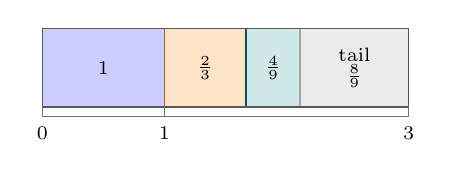
\begin{tikzpicture}[
  x=1.55cm,
  y=1.0cm,
  every node/.style={font=\scriptsize},
  frame/.style={draw=black!65, line width=0.65pt},
  stripa/.style={fill=blue!20, draw=blue!65!black, line width=0.55pt},
  stripb/.style={fill=orange!22, draw=orange!75!black, line width=0.55pt},
  stripc/.style={fill=teal!18, draw=teal!70!black, line width=0.55pt},
  tail/.style={fill=gray!16, draw=gray!70, line width=0.55pt},
  axis/.style={black!55, line width=0.45pt}
]
  \draw[stripa] (0,0) rectangle (1,1);
  \draw[stripb] (1,0) rectangle (1.6667,1);
  \draw[stripc] (1.6667,0) rectangle (2.1111,1);
  \draw[tail] (2.1111,0) rectangle (3,1);
  \draw[frame] (0,0) rectangle (3,1);

  \foreach \x/\lab in {0/0,1/1,3/3} {
    \draw[axis] (\x,0) -- (\x,-0.12);
    \node[below] at (\x,-0.12) {$\lab$};
  }
  \draw[axis] (0,-0.12) -- (3,-0.12);

  \node at (0.5,0.5) {$1$};
  \node at (1.333,0.5) {$\frac23$};
  \node at (1.889,0.5) {$\frac49$};
  \node[align=center] at (2.556,0.5) {tail\\[-1pt]$\frac89$};
\end{tikzpicture}

  \caption{At $x=\frac{2}{3}$, the strip widths sum to $1+\frac{2}{3}+\frac{4}{9}+\cdots=3$.}
  \label{fig:geometric-series-rectangle-two-thirds}
\end{illustrationfigure}

\begin{definition} \label{def:real-decimal-as-series} \hlt{Real Decimals as Series}\\
Let $N\in\N_0$, $b_N,\ldots,b_0,a_1,a_2,\ldots\in\{0,\ldots,9\}$; $b_N\neq0$ unless integer part is $0$. Define $b_N\cdots b_0.a_1a_2\cdots\defeq\sum\limits_{i=0}^{N}b_i10^i+\sum\limits_{j=1}^{\infty}a_j10^{-j}$.\\
The fractional series converges absolutely by Theorems \ref{thm:series-comparison-test}(i) and \ref{thm:geometric-series-nonnegative}(i), since $(\forall j\in\N)\,0\leq a_j10^{-j}\leq10^{1-j}$.\\
A prefixed minus sign denotes the negative of this value.
\end{definition}

\begin{proposition} \label{prop:decimal-terminal-nine-nonuniqueness} \hlt{Terminal Nines Are Nonunique}\\
The same real number can have two decimal representations: $1.000\ldots=0.999\ldots$.
\begin{proof}
$1.000\ldots=1+\sum\limits_{j=1}^{\infty}0\cdot10^{-j}=1$, while $0.999\ldots=\sum\limits_{j=1}^{\infty}9\cdot10^{-j}=9\frac{10^{-1}}{1-10^{-1}}=1$ by Theorem \ref{thm:geometric-series-nonnegative}(i).\\
\hlt{Structural Commentary}: The geometric-tail calculation identifies the limits of the two decimal partial-sum sequences.\\
\hlt{Key Insight}: Repeated $9$s exactly fill the preceding decimal gap.
\end{proof}
\end{proposition}

\begin{perspective} \label{per:decimal-expansions-as-series} \hlt{Decimal Expansions Are Series}\\
Proposition \ref{prop:decimal-truncations-squeeze-real} constructs decimal truncations converging to a real number, while Definition \ref{def:real-decimal-as-series} interprets the infinite digit string as a series. Proposition \ref{prop:decimal-terminal-nine-nonuniqueness} identifies the standard terminal-$9$ ambiguity.
\end{perspective}

\begin{theorem} \label{thm:cauchy-condensation-test} \hlt{Cauchy Condensation Test}\\
Let $(a_n)_{n\geq1}\subseteq[0,\infty)$ satisfy $a_1\geq a_2\geq\cdots$. Then $\sum\limits_{n=1}^{\infty}a_n$ converges iff $\sum\limits_{k=0}^{\infty}2^k a_{2^k}$ converges.
\begin{proof}
Let $s_n\defeq\sum\limits_{j=1}^{n}a_j$ and $t_k\defeq\sum\limits_{j=0}^{k}2^j a_{2^j}$. Both partial-sum sequences are nondecreasing.
\begin{enumerate}[label=\roman*.]
\setlength{\itemsep}{0pt}
\item[$(\Rightarrow)$] If $(s_n)$ is bounded, then $t_m\leq2\sum\limits_{j=1}^{2^m}a_j=2s_{2^m}$, so $(t_m)$ is bounded and the condensed series converges by Theorem \ref{thm:nonnegative-series-bounded-partial-sums}.
\item[$(\Leftarrow)$] If $(t_k)$ bounded, then for $2^m\leq n<2^{m+1}$, $s_n\leq\sum\limits_{j=0}^{m}2^j a_{2^j}=t_m$; $(s_n)$ bounded, original series converges by Theorem \ref{thm:nonnegative-series-bounded-partial-sums}.
\end{enumerate}
\hlt{Structural Commentary}: Monotonicity bounds each dyadic block by an endpoint value, transferring bounded partial sums both ways.\\
\hlt{Key Insight}: Dyadic blocks preserve the convergence threshold.
\end{proof}
\end{theorem}

\begin{corollary} \label{cor:p-series-test} \hlt{$p$-Series Test}\\
For $p\in\R$:
\begin{enumerate}[label=(\roman*)]
\setlength{\itemsep}{0pt}
\item If $p>1$, then $\sum\limits_{n=1}^{\infty}n^{-p}$ converges.
\item If $p\leq1$, then $\sum\limits_{n=1}^{\infty}n^{-p}$ diverges.
\end{enumerate}
\begin{proof}
\begin{enumerate}[label=(\roman*)]
\setlength{\itemsep}{0pt}
\item If $p>1$, the condensed series is $\sum\limits_{k=0}^{\infty}2^k(2^k)^{-p}=\sum\limits_{k=0}^{\infty}2^{(1-p)k}$, which converges by Theorem \ref{thm:geometric-series-nonnegative}(i) because $2^{1-p}<1$.\\
Thus the original series converges by Theorem \ref{thm:cauchy-condensation-test}.
\item If $p\leq0$, then $n^{-p}\not\to0$, so the series diverges by Corollary \ref{cor:series-terms-tend-to-zero}.\\
If $0<p\leq1$, the condensed geometric series has ratio $2^{1-p}\geq1$, so the original series diverges by Theorems \ref{thm:cauchy-condensation-test} and \ref{thm:geometric-series-nonnegative}(ii).
\end{enumerate}
\hlt{Structural Commentary}: Condensation converts the power law $n^{-p}$ into the geometric ratio $2^{1-p}$.\\
\hlt{Key Insight}: The threshold occurs at $2^{1-p}=1$.
\end{proof}
\end{corollary}

\begin{theorem} \label{thm:integral-test-series} \hlt{Integral Test}\\
Let $N\in\N$ and let $f:[N,\infty)\to[0,\infty)$ be decreasing and Riemann integrable on every compact subinterval.
\begin{enumerate}[label=(\roman*)]
\setlength{\itemsep}{0pt}
\item $(\forall M\in\N)\,[M\geq N\Rightarrow\int_N^{M+1}f(x)\,dx\leq\sum\limits_{k=N}^{M}f(k)\leq f(N)+\int_N^M f(x)\,dx]$.
\item $\sum\limits_{k=N}^{\infty}f(k)$ converges iff $\int_N^\infty f(x)\,dx$ converges.
\end{enumerate}
\begin{proof}
\begin{enumerate}[label=(\roman*)]
\setlength{\itemsep}{0pt}
\item[$(i)$] For $x\in[k,k+1]$, $f(x)\leq f(k)$, so $\int_N^{M+1}f\leq\sum\limits_{k=N}^{M}f(k)$.\\
For $k\geq N+1$ and $x\in[k-1,k]$, $f(k)\leq f(x)$, so $\sum\limits_{k=N}^{M}f(k)\leq f(N)+\int_N^M f$.
\item[$(ii)$] ($\Rightarrow$) If $\sum\limits_{k=N}^{\infty}f(k)$ converges, its partial sums are bounded.\\
For $d\geq N$, choose $M\in\N$ with $M\geq N$ and $d\leq M+1$; then $0\leq\int_N^d f\leq\int_N^{M+1}f\leq\sum\limits_{k=N}^{M}f(k)$ by (i).\\
Thus the nonnegative truncation integrals are bounded, so $\int_N^\infty f$ converges by Theorem \ref{thm:nonnegative-improper-integral-supremum}(ii).
\item[$(ii)$] ($\Leftarrow$) If $\int_N^\infty f$ converges, its nonnegative truncation integrals are bounded by Theorem \ref{thm:nonnegative-improper-integral-supremum}(ii).\\
The partial sums $\sum\limits_{k=N}^{M}f(k)$ are then bounded by (i), so the series converges by Theorem \ref{thm:nonnegative-series-bounded-partial-sums}.
\end{enumerate}
\hlt{Structural Commentary}: Monotonicity sandwiches unit-interval areas between samples, transferring boundedness of the two truncations.\\
\hlt{Key Insight}: Series mass and integral area differ by at most one endpoint term.
\end{proof}
\end{theorem}

Figure \ref{fig:integral-test-step-functions} shows the endpoint rectangles underlying the bounds in Theorem \ref{thm:integral-test-series}(i).

\begin{illustrationfigure}[H]
  \centering
  \begin{tikzpicture}[
  x=0.78cm,
  y=0.72cm,
  >=Stealth,
  every node/.style={font=\scriptsize},
  axis/.style={->, black!55, line width=0.45pt},
  curve/.style={black!85, line width=0.9pt},
  upper/.style={draw=black!55, line width=0.45pt},
  lower/.style={fill=gray!18, draw=black!55, line width=0.45pt},
  guide/.style={black!18, dashed, line width=0.35pt}
]
  \draw[axis] (-0.25,0) -- (5.65,0) node[right] {$x$};
  \draw[axis] (0,-0.15) -- (0,3.20);

  \foreach \x in {0,1,2,3,4,5} {
    \draw[guide] (\x,0) -- (\x,3.0);
  }
  \foreach \x/\lab in {0/$N$,1/$N+1$,4/$M$,5/$M+1$} {
    \node[below] at (\x,0) {\lab};
  }
  \node[below] at (2.55,0) {$\cdots$};

  \foreach \xl/\xr in {0/1,1/2,2/3,3/4,4/5} {
    \pgfmathsetmacro{\hleft}{2.55/(1+0.42*\xl)+0.35}
    \pgfmathsetmacro{\hright}{2.55/(1+0.42*\xr)+0.35}
    \draw[lower] (\xl,0) rectangle (\xr,\hright);
    \draw[upper] (\xl,0) rectangle (\xr,\hleft);
  }

  \draw[curve, domain=0:5.15, samples=120]
    plot (\x,{2.55/(1+0.42*\x)+0.35}) node[right] {$f$};
\end{tikzpicture}

  \caption{Left and right endpoint estimates for decreasing $f\geq0$.}
  \label{fig:integral-test-step-functions}
\end{illustrationfigure}

\begin{definition} \label{def:number-e-by-series} \hlt{The Number $e$}\\
Define $e\defeq\sum\limits_{n=0}^{\infty}\frac{1}{n!}$, where $0!\defeq1$. Since $(\forall n\in\N)\,n!=\prod\limits_{k=1}^{n}k\geq2^{n-1}$, defining series converges by Theorems \ref{thm:series-comparison-test}(i), \ref{thm:geometric-series-nonnegative}(i).
\end{definition}

\begin{theorem} \label{thm:e-as-binomial-limit} \hlt{A Limit Formula for $e$}\\
The limit formula is $\lim\limits_{n\to\infty}\left(1+\frac{1}{n}\right)^n=e$.
\begin{proof}
Set $s_m\defeq\sum\limits_{k=0}^{m}\frac{1}{k!}$ and $t_n\defeq\left(1+\frac{1}{n}\right)^n$. By Proposition \ref{prop:binomial-theorem-and-subset-count}(i), $t_n=1+\sum\limits_{k=1}^{n}\frac{1}{k!}\prod\limits_{j=0}^{k-1}\left(1-\frac{j}{n}\right)\leq s_n$.\\
Thus $\limsup\limits_{n\to\infty}t_n\leq e$ by Theorems \ref{thm:limsup-liminf-order-comparison}(i) and \ref{thm:convergence-iff-limsup-liminf-equal}. Fix $m\in\N$. For $n\geq m$, let $u_n^{(m)}\defeq1+\sum\limits_{k=1}^{m}\frac{1}{k!}\prod\limits_{j=0}^{k-1}\left(1-\frac{j}{n}\right)\leq t_n$.\\
Then $u_n^{(m)}\to s_m$ by repeated application of Theorem \ref{thm:complex-sequence-limit-algebra}. Thus $s_m\leq\liminf\limits_{n\to\infty}t_n$ by Theorems \ref{thm:limsup-liminf-order-comparison}(ii) and \ref{thm:convergence-iff-limsup-liminf-equal}.\\
Since $s_m\to e$, $e\leq\liminf\limits_{n\to\infty}t_n\leq\limsup\limits_{n\to\infty}t_n\leq e$ by Definition \ref{def:upper-and-lower-limits}; hence $t_n\to e$ by Theorem \ref{thm:convergence-iff-limsup-liminf-equal}.\\
\hlt{Structural Commentary}: Full factorial truncations bound $t_n$ above, while each fixed truncation bounds its liminf below.\\
\hlt{Key Insight}: Fix the truncation before sending $n\to\infty$.
\end{proof}
\end{theorem}

\begin{proposition} \label{prop:e-series-remainder-bound} \hlt{Remainder Bound for the Series of $e$}\\
If $n\geq1$ and $s_n=\sum\limits_{k=0}^{n}\frac{1}{k!}$, then $0<e-s_n<\frac{1}{n!\,n}$.
\begin{proof}
For $j\geq1$, $\frac{1}{(n+j)!}\leq\frac{1}{(n+1)!}\left(\frac{1}{n+1}\right)^{j-1}$,  strict inequality for $j\geq2$; $0<e-s_n<\frac{1}{(n+1)!}\sum\limits_{j=0}^{\infty}\left(\frac{1}{n+1}\right)^j=\frac{1}{n!\,n}$ by Theorem \ref{thm:geometric-series-nonnegative}(i).\\
\hlt{Structural Commentary}: Successive factorial denominators dominate a geometric tail with ratio $\frac{1}{n+1}$.\\
\hlt{Key Insight}: The factorial tail is smaller than its geometric majorant.
\end{proof}
\end{proposition}

\begin{theorem} \label{thm:e-irrational} \hlt{$e$ Is Irrational}\\
The number $e$ is irrational.
\begin{proof}
Suppose $e=\frac{p}{q}$ with $p,q\in\N$. By Proposition \ref{prop:e-series-remainder-bound}, $0<q!(e-s_q)<\frac{1}{q}\leq1$.\\
But $q!e$ and $q!s_q$ are integers, so $q!(e-s_q)$ is an integer strictly between $0$ and $1$, impossible.\\
\hlt{Structural Commentary}: Clearing a hypothetical denominator turns the factorial-tail bound into an impossible integer interval.\\
\hlt{Key Insight}: No integer lies strictly between $0$ and $1$.
\end{proof}
\end{theorem}

\begin{theorem} \label{thm:root-test} \hlt{Root Test}\\
For $(a_n)_{n\geq1}\subseteq\C$, put $\alpha\defeq\limsup\limits_{n\to\infty}\sqrt[n]{\abs{a_n}}$. Then:
\begin{enumerate}[label=(\roman*)]
\setlength{\itemsep}{0pt}
\item if $\alpha<1$, then $\sum a_n$ converges absolutely;
\item if $\alpha>1$, then $\sum a_n$ diverges;
\item if $\alpha=1$, the test is inconclusive.
\end{enumerate}
\begin{proof}
\begin{enumerate}[label=(\roman*)]
\setlength{\itemsep}{0pt}
\item Choose $\alpha<\beta<1$. By Theorem \ref{thm:limsup-characterization}(ii), choose $N\in\N$ such that $(\forall n\geq N)\,\sqrt[n]{\abs{a_n}}<\beta$, hence $(\forall n\geq N)\,\abs{a_n}<\beta^n$.\\
Thus $\sum\abs{a_n}$ converges by Theorems \ref{thm:series-comparison-test}(i) and \ref{thm:geometric-series-nonnegative}(i).
\item Since $\alpha>1$, $\abs{a_n}>1$ for infinitely many $n$ by Theorem \ref{thm:limsup-characterization}(i), so $a_n\not\to0$ and the series diverges by Corollary \ref{cor:series-terms-tend-to-zero}.
\item The relations $\sqrt[n]{n^{-1}}=(\sqrt[n]{n})^{-1}\to1$ and $\sqrt[n]{n^{-2}}=(\sqrt[n]{n})^{-2}\to1$ hold by Theorem \ref{thm:special-sequence-limits}(iii) and Theorem \ref{thm:complex-sequence-limit-algebra}.\\
The two series have different behavior by Corollary \ref{cor:p-series-test}, so $\alpha=1$ determines neither convergence nor divergence.
\end{enumerate}
\hlt{Structural Commentary}: Limsup bounds roots by a geometric ratio, while roots above $1$ obstruct vanishing terms.\\
\hlt{Key Insight}: The threshold $1$ separates geometric decay from persistent terms.
\end{proof}
\end{theorem}

\begin{theorem} \label{thm:ratio-test} \hlt{Ratio Test}\\
Let $(a_n)_{n\geq1}\subseteq\C$ and assume $(\exists N_0\in\N)(\forall n\geq N_0)\,a_n\neq0$.
\begin{enumerate}[label=(\roman*)]
\setlength{\itemsep}{0pt}
\item If $\limsup\limits_{n\to\infty}\abs{\frac{a_{n+1}}{a_n}}<1$, then $\sum a_n$ converges absolutely.
\item If $\liminf\limits_{n\to\infty}\abs{\frac{a_{n+1}}{a_n}}>1$, then $\sum a_n$ diverges.
\item In the remaining cases, the test is inconclusive.
\end{enumerate}
\begin{proof}
\begin{enumerate}[label=(\roman*)]
\setlength{\itemsep}{0pt}
\item Choose $\beta$ with $\limsup\limits_{n\to\infty}\abs{\frac{a_{n+1}}{a_n}}<\beta<1$. By Theorem \ref{thm:limsup-characterization}(ii), choose $N\geq N_0$ such that $(\forall n\geq N)\,\abs{a_{n+1}}\leq\beta\abs{a_n}$.\\
Then $(\forall n\geq N)\,\abs{a_n}\leq\abs{a_N}\beta^{n-N}$, so $\sum\abs{a_n}$ converges by Theorems \ref{thm:series-comparison-test}(i) and \ref{thm:geometric-series-nonnegative}(i).
\item Choose $\beta$ with $1<\beta<\liminf\limits_{n\to\infty}\abs{\frac{a_{n+1}}{a_n}}$. By Theorem \ref{thm:limsup-characterization}(v), choose $N\geq N_0$ such that $(\forall n\geq N)\,\abs{a_{n+1}}>\beta\abs{a_n}$.\\
Thus $(\forall n\geq N)\,\abs{a_n}\geq\abs{a_N}>0$, so the series diverges by Corollary \ref{cor:series-terms-tend-to-zero}.
\item Set $r_n\defeq\frac{n}{n+1}=\left(1+\frac{1}{n}\right)^{-1}\to1$ by Theorems \ref{thm:special-sequence-limits}(i) and \ref{thm:complex-sequence-limit-algebra}.\\
The term ratios of $\sum\frac{1}{n}$ and $\sum\frac{1}{n^2}$ are respectively $r_n$ and $r_n^2$, so both tend to $1$ by Theorem \ref{thm:complex-sequence-limit-algebra}.\\
The two series have different behavior by Corollary \ref{cor:p-series-test}.
\end{enumerate}
\hlt{Structural Commentary}: An eventual ratio bound iterates to a geometric majorant or to a positive lower bound.\\
\hlt{Key Insight}: Successive ratios control the entire tail by induction.
\end{proof}
\end{theorem}

\begin{theorem} \label{thm:root-test-dominates-ratio-test} \hlt{Root and Ratio Test Comparison}\\
For $(c_n)_{n\geq1}\subseteq(0,\infty)$:
\begin{enumerate}[label=(\roman*)]
\setlength{\itemsep}{0pt}
\item $\liminf\limits_{n\to\infty}\frac{c_{n+1}}{c_n}\leq \liminf\limits_{n\to\infty}\sqrt[n]{c_n}$;
\item $\liminf\limits_{n\to\infty}\sqrt[n]{c_n}\leq \limsup\limits_{n\to\infty}\sqrt[n]{c_n}$;
\item $\limsup\limits_{n\to\infty}\sqrt[n]{c_n}\leq \limsup\limits_{n\to\infty}\frac{c_{n+1}}{c_n}$.
\end{enumerate}
\begin{proof}
\begin{enumerate}[label=(\roman*)]
\setlength{\itemsep}{0pt}
\item Let $\ell\defeq\liminf\limits_{n\to\infty}\frac{c_{n+1}}{c_n}$. If $\ell=0$, the inequality is automatic.\\
For $0<\gamma<\ell$, choose $N\in\N$ such that $(\forall n\geq N)\,c_{n+1}\geq\gamma c_n$ by Theorem \ref{thm:limsup-characterization}(v).\\
Hence $(\forall n\geq N)\,c_n\geq c_N\gamma^{n-N}$. The lower bound has $n$th-root limit $\gamma$ by Theorem \ref{thm:special-sequence-limits}(ii), so $\liminf\limits_{n\to\infty}\sqrt[n]{c_n}\geq\gamma$; let $\gamma\uparrow\ell$.
\item The inequality holds by Definition \ref{def:upper-and-lower-limits} because the infimum of the subsequential-limit set does not exceed its supremum.
\item Let $\alpha\defeq\limsup\limits_{n\to\infty}\frac{c_{n+1}}{c_n}$. If $\alpha=+\infty$, the inequality is automatic.\\
If $\alpha<+\infty$ and $\beta>\alpha$, choose $N\in\N$ such that $(\forall n\geq N)\,c_{n+1}\leq\beta c_n$ by Theorem \ref{thm:limsup-characterization}(ii).\\
Hence $(\forall n\geq N)\,c_n\leq c_N\beta^{n-N}$. The upper bound has $n$th-root limit $\beta$ by Theorem \ref{thm:special-sequence-limits}(ii), so $\limsup\limits_{n\to\infty}\sqrt[n]{c_n}\leq\beta$; let $\beta\downarrow\alpha$.
\end{enumerate}
\hlt{Structural Commentary}: Eventual ratio bounds telescope into geometric bounds whose $n$th roots retain the same ratio.\\
\hlt{Key Insight}: Multiplicative tail control survives passage to $n$th roots.
\end{proof}
\end{theorem}

\begin{theorem} \label{thm:summation-by-parts} \hlt{Summation by Parts}\\
Let $(a_n)_{n\geq0},(b_n)_{n\geq0}\subseteq\C$, $A_{-1}\defeq0$, and $A_n\defeq\sum\limits_{k=0}^{n}a_k$. For integers $0\leq p\leq q$, $\sum\limits_{n=p}^{q}a_nb_n=\sum\limits_{n=p}^{q-1}A_n(b_n-b_{n+1})+A_qb_q-A_{p-1}b_p$.
\begin{proof}
By $a_n=A_n-A_{n-1}$, $\sum\limits_{n=p}^{q}a_nb_n=\sum\limits_{n=p}^{q}A_nb_n-\sum\limits_{n=p}^{q}A_{n-1}b_n$.\\
Reindexing the second sum implies $\sum\limits_{n=p}^{q}a_nb_n=\sum\limits_{n=p}^{q-1}A_n(b_n-b_{n+1})+A_qb_q-A_{p-1}b_p$.\\
\hlt{Structural Commentary}: Substituting $a_n=A_n-A_{n-1}$ and reindexing makes the interior terms telescope.\\
\hlt{Key Insight}: Reindexing transfers the discrete difference from $A_n$ to $b_n$.
\end{proof}
\end{theorem}

\begin{theorem} \label{thm:dirichlet-test-series} \hlt{Dirichlet Test}\\
Let $(a_n)_{n\geq1}\subseteq\C$ and $(b_n)_{n\geq1}\subseteq[0,\infty)$. Set $A_0\defeq0$ and $A_n\defeq\sum\limits_{k=1}^{n}a_k$. If $(A_n)$ is bounded and $b_n\downarrow0$, then $\sum a_nb_n$ converges.
\begin{proof}
Extend the sequences by $a_0\defeq0$ and $b_0\defeq b_1$, so Theorem \ref{thm:summation-by-parts} applies without changing $A_n$ for $n\geq1$.\\
Fix $\varepsilon>0$ and choose $M>0$ such that $(\forall n\in\N_0)\,\abs{A_n}\leq M$. Choose $N\in\N$ such that $b_N<\frac{\varepsilon}{2M}$.\\
For $N\leq p\leq q$, $\abs{\sum\limits_{n=p}^{q}a_nb_n}\leq M\left(\sum\limits_{n=p}^{q-1}(b_n-b_{n+1})+b_q+b_p\right)=2Mb_p\leq2Mb_N<\varepsilon$ by Theorem \ref{thm:summation-by-parts}.\\
Thus $\sum a_nb_n$ converges by Theorem \ref{thm:series-cauchy-criterion}.\\
\hlt{Structural Commentary}: Summation by parts combines bounded partial sums with the telescoping variation of decreasing $b_n$.\\
\hlt{Key Insight}: Monotone decay converts cancellation into the bound $2Mb_p$.
\end{proof}
\end{theorem}

\begin{corollary} \label{cor:alternating-series-test} \hlt{Alternating Series Test}\\
Let $(c_n)_{n\geq1}\subseteq\R$ satisfy $(\forall n\in\N)\,\abs{c_{n+1}}\leq\abs{c_n}$ and $c_n\to0$. If $(\exists\sigma\in\{-1,1\})(\forall n\in\N)\,c_n=\sigma(-1)^{n+1}\abs{c_n}$, then $\sum c_n$ converges.
\begin{proof}
Choose $\sigma\in\{-1,1\}$ from hypothesis. Partial sums of $(\sigma(-1)^{n+1})$ bounded, while $\abs{c_n}\downarrow0$, so $\sum c_n$ converges by Theorem \ref{thm:dirichlet-test-series}.\\
\hlt{Structural Commentary}: Alternating signs supply bounded partial sums, and decreasing magnitudes meet Dirichlet's damping condition.\\
\hlt{Key Insight}: Alternation is the simplest source of bounded cancellation.
\end{proof}
\end{corollary}

\begin{perspective} \label{per:alternating-series-interval-picture} \hlt{Alternating Partial Sums as Nested Control}\\
Set $a_n\defeq\abs{c_n}$. Figure \ref{fig:alternating-series-intervals} depicts $I_j=[a_{2j},a_{2j-1}]$, whose interiors are pairwise disjoint.\\
Their lengths are the paired terms in the even partial sums, so those sums stay in $[0,a_1]$.\\
Each odd partial sum differs by the next term, which tends to $0$.
\end{perspective}

\begin{illustrationfigure}[H]
  \centering
  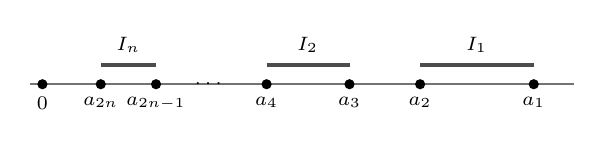
\begin{tikzpicture}[
  x=0.78cm,
  y=0.72cm,
  every node/.style={font=\scriptsize},
  axis/.style={black!55, line width=0.55pt},
  point/.style={circle, fill=black, inner sep=1.3pt},
  interval/.style={black!70, line width=1.2pt}
]
  \draw[axis] (-0.2,0) -- (8.65,0);

  \foreach \x/\lab in {
    0/$0$,
    0.95/a_{2n},
    1.85/a_{2n-1},
    3.65/a_4,
    5.00/a_3,
    6.15/a_2,
    8.00/a_1
  } {
    \node[point] at (\x,0) {};
    \node[below] at (\x,-0.05) {$\lab$};
  }

  \draw[interval] (0.95,0.34) -- (1.85,0.34);
  \draw[interval] (3.65,0.34) -- (5.00,0.34);
  \draw[interval] (6.15,0.34) -- (8.00,0.34);

  \node[above] at (1.40,0.38) {$I_n$};
  \node[above] at (4.32,0.38) {$I_2$};
  \node[above] at (7.07,0.38) {$I_1$};

  \node at (2.70,0) {$\cdots$};
\end{tikzpicture}

  \caption{For $a_n\defeq\abs{c_n}$, the ordered intervals $I_j=[a_{2j},a_{2j-1}]$ have pairwise disjoint interiors in $[0,a_1]$.}
  \label{fig:alternating-series-intervals}
\end{illustrationfigure}

Set $s\defeq\sum\limits_{k=1}^{\infty}\frac{(-1)^{k+1}}{k}$, which exists by Corollary \ref{cor:alternating-series-test}. Figure \ref{fig:alternating-harmonic-partial-sums} plots $s_n=\sum\limits_{k=1}^{n}\frac{(-1)^{k+1}}{k}$ vertically against the dimensionless integer index $n$ for $1\leq n\leq10$; its dashed reference level is $s$.

\begin{visualizationfigure}[H]
  \centering
  \begin{tikzpicture}[
  >=Stealth,
  x=0.72cm,
  y=3.0cm,
  every node/.style={font=\scriptsize},
  axis/.style={->, gray!70, line width=0.55pt},
  odd/.style={blue!70!black, line width=0.9pt},
  even/.style={orange!85!black, line width=0.9pt},
  limit/.style={black!60, dashed, line width=0.6pt},
  pointodd/.style={circle, fill=blue!70!black, inner sep=1.35pt},
  pointeven/.style={circle, fill=orange!85!black, inner sep=1.35pt}
]
  \draw[axis] (0.35,0.43) -- (10.25,0.43) node[right] {$n$};
  \draw[axis] (0.7,0.43) -- (0.7,1.07) node[above] {$s_n$};
  \draw[limit] (0.82,0.693) -- (9.75,0.693)
    node[right, black] {$\log 2$};

  \draw[odd] plot coordinates {(1,1.000) (3,0.833) (5,0.783) (7,0.760) (9,0.746)};
  \draw[even] plot coordinates {(2,0.500) (4,0.583) (6,0.617) (8,0.635) (10,0.646)};

  \foreach \x/\y in {1/1.000,3/0.833,5/0.783,7/0.760,9/0.746} {
    \node[pointodd] at (\x,\y) {};
  }
  \foreach \x/\y in {2/0.500,4/0.583,6/0.617,8/0.635,10/0.646} {
    \node[pointeven] at (\x,\y) {};
  }
\end{tikzpicture}

  \caption{Odd partial sums (blue) decrease and even partial sums (orange) increase toward the series sum $s$.}
  \label{fig:alternating-harmonic-partial-sums}
\end{visualizationfigure}

\begin{theorem} \label{thm:absolute-convergence-implies-convergence} \hlt{Absolute Convergence Implies Convergence}\\
If $\sum a_n$ converges absolutely, then $\sum a_n$ converges.
\begin{proof}
The series $\sum a_n$ converges by Theorem \ref{thm:series-comparison-test}(i) with $c_n\defeq\abs{a_n}$.\\
\hlt{Structural Commentary}: The comparison test transfers convergence from the modulus series to the original complex series.\\
\hlt{Key Insight}: Absolute convergence is self-majorization by $\abs{a_n}$.
\end{proof}
\end{theorem}

\begin{theorem} \label{thm:linearity-of-convergent-series} \hlt{Addition and Scalar Multiplication of Series}
\begin{enumerate}[label=(\roman*)]
\setlength{\itemsep}{0pt}
\item If $\sum a_n=A$ and $\sum b_n=B$, then $\sum(a_n+b_n)=A+B$.
\item If $\sum a_n=A$ and $c\in\C$, then $\sum ca_n=cA$.
\end{enumerate}
\begin{proof}
\begin{enumerate}[label=(\roman*)]
\setlength{\itemsep}{0pt}
\item If $s_N\defeq\sum\limits_{n=1}^{N}a_n$ and $t_N\defeq\sum\limits_{n=1}^{N}b_n$, then $\sum\limits_{n=1}^{N}(a_n+b_n)=s_N+t_N\to A+B$ by Theorem \ref{thm:complex-sequence-limit-algebra}(i).
\item If $s_N\defeq\sum\limits_{n=1}^{N}a_n$, then $\sum\limits_{n=1}^{N}ca_n=cs_N\to cA$ by Theorem \ref{thm:complex-sequence-limit-algebra}(ii).
\end{enumerate}
\hlt{Structural Commentary}: Finite-sum identities reduce both claims to limit algebra for the corresponding partial-sum sequences.\\
\hlt{Key Insight}: Series linearity is sequence linearity of partial sums.
\end{proof}
\end{theorem}

\begin{definition} \label{def:cauchy-product-of-series} \hlt{Cauchy Product}\\
For series $\sum\limits_{n=0}^{\infty}a_n$ and $\sum\limits_{n=0}^{\infty}b_n$, set $c_n\defeq\sum\limits_{k=0}^{n}a_kb_{n-k}$ for $n\in\N_0$. The series $\sum\limits_{n=0}^{\infty}c_n$ is their \hlt{Cauchy product}.
\end{definition}

Figure \ref{fig:cauchy-product-diagonals} groups the array entries $a_i b_j$ by diagonals $i+j=n$, matching the definition of each coefficient $c_n$.

\begin{illustrationfigure}[H]
  \centering
  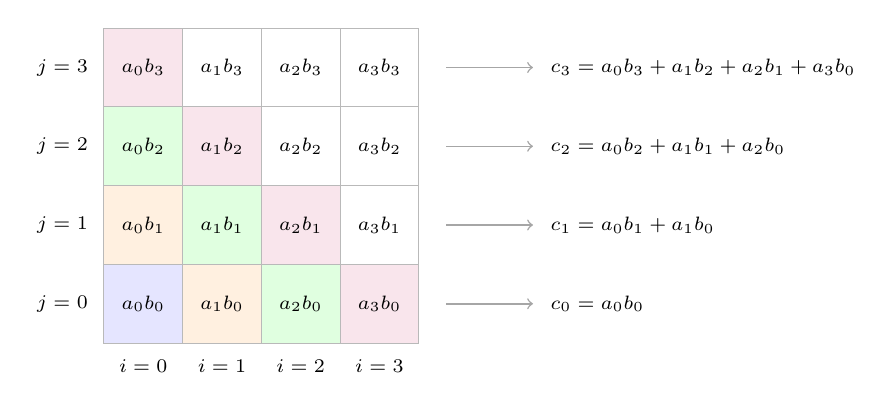
\begin{tikzpicture}[
  every node/.style={font=\scriptsize},
  cell/.style={draw=gray!55, line width=0.35pt},
  diagA/.style={fill=blue!10},
  diagB/.style={fill=orange!12},
  diagC/.style={fill=green!12},
  diagD/.style={fill=purple!10},
  arrow/.style={->, gray!70, line width=0.55pt}
]
  \foreach \i in {0,1,2,3} {
    \foreach \j in {0,1,2,3} {
      \pgfmathtruncatemacro{\diagindex}{\i+\j}
      \ifnum\diagindex=0
        \path[diagA] (\i,\j) rectangle ++(1,1);
      \fi
      \ifnum\diagindex=1
        \path[diagB] (\i,\j) rectangle ++(1,1);
      \fi
      \ifnum\diagindex=2
        \path[diagC] (\i,\j) rectangle ++(1,1);
      \fi
      \ifnum\diagindex=3
        \path[diagD] (\i,\j) rectangle ++(1,1);
      \fi
      \draw[cell] (\i,\j) rectangle ++(1,1);
      \node at (\i+0.5,\j+0.5) {$a_{\i}b_{\j}$};
    }
  }

  \foreach \i in {0,1,2,3} {
    \node[below] at (\i+0.5,-0.08) {$i=\i$};
    \node[left] at (-0.08,\i+0.5) {$j=\i$};
  }

  \draw[arrow] (4.35,0.5) -- (5.45,0.5);
  \node[right, align=left] at (5.55,0.5) {$c_0=a_0b_0$};

  \draw[arrow] (4.35,1.5) -- (5.45,1.5);
  \node[right, align=left] at (5.55,1.5) {$c_1=a_0b_1+a_1b_0$};

  \draw[arrow] (4.35,2.5) -- (5.45,2.5);
  \node[right, align=left] at (5.55,2.5) {$c_2=a_0b_2+a_1b_1+a_2b_0$};

  \draw[arrow] (4.35,3.5) -- (5.45,3.5);
  \node[right, align=left] at (5.55,3.5) {$c_3=a_0b_3+a_1b_2+a_2b_1+a_3b_0$};

\end{tikzpicture}

  \caption{Diagonal sums of $(a_i b_j)$ form the Cauchy product; finite rectangular sums are order-free.}
  \label{fig:cauchy-product-diagonals}
\end{illustrationfigure}

\begin{theorem} \label{thm:mertens-cauchy-product} \hlt{Mertens' Theorem for Cauchy Products}\\
Suppose $\sum\limits_{n=0}^{\infty}a_n=A$ converges absolutely, $\sum\limits_{n=0}^{\infty}b_n=B$, and $c_n\defeq\sum\limits_{k=0}^{n}a_kb_{n-k}$. Then $\sum\limits_{n=0}^{\infty}c_n=AB$.
\begin{proof}
\begin{enumerate}[label=(\roman*)]
\setlength{\itemsep}{0pt}
\item \hlt{Setup}: Set $A_n\defeq\sum\limits_{k=0}^{n}a_k$, $B_n\defeq\sum\limits_{k=0}^{n}b_k$, $C_n\defeq\sum\limits_{k=0}^{n}c_k$, and $\beta_n\defeq B_n-B$.
\item \hlt{Error Decomposition}: Finite reindexing implies $C_n=\sum\limits_{k=0}^{n}a_kB_{n-k}=A_nB+\gamma_n$, where $\gamma_n\defeq\sum\limits_{k=0}^{n}a_k\beta_{n-k}$.\\
Since $A_nB\to AB$ by Theorem \ref{thm:complex-sequence-limit-algebra}(ii), it suffices to prove $\gamma_n\to0$.
\item \hlt{Tail Estimate}: Put $\alpha\defeq\sum\limits_{n=0}^{\infty}\abs{a_n}$. Fix $\varepsilon>0$ and choose $N\in\N_0$ such that $(\forall j\geq N)\,\abs{\beta_j}<\frac{\varepsilon}{2(\alpha+1)}$.\\
Then $\abs{\gamma_n}\leq\abs{\sum\limits_{j=0}^{N}\beta_j a_{n-j}}+\frac{\varepsilon\alpha}{2(\alpha+1)}<\abs{\sum\limits_{j=0}^{N}\beta_j a_{n-j}}+\frac{\varepsilon}{2}$ for $n\geq N$.
\item \hlt{Conclusion}: For fixed $N$, $\sum\limits_{j=0}^{N}\beta_j a_{n-j}\to0$ by Corollary \ref{cor:series-terms-tend-to-zero}, Theorem \ref{thm:complex-sequence-limit-algebra}. Thus $\abs{\gamma_n}<\varepsilon$, so $\gamma_n\to0$ and $C_n\to AB$.
\end{enumerate}
\hlt{Structural Commentary}: Splitting the convolution error at a fixed index combines finitely many vanishing terms with an absolute tail.\\
\hlt{Key Insight}: One absolutely summable factor controls every convolution error.
\end{proof}
\end{theorem}

\begin{perspective} \label{per:cauchy-product-diagonal-ordering} \hlt{Diagonal Ordering in a Product}\\
Coefficient $c_n$ is diagonal sum of products $a_i b_j$ with $i+j=n$. Theorem \ref{thm:mertens-cauchy-product} controls this diagonal ordering when one factor converges absolutely; it does not assert invariance under arbitrary reorderings of the double array.
\end{perspective}

\begin{definition} \label{def:series-rearrangement} \hlt{Rearrangement of a Series}\\
Let $\pi:\N\to\N$ be bijective and set $a'_n\defeq a_{\pi(n)}$. Then $\sum a'_n$ is a \hlt{rearrangement} of $\sum a_n$.
\end{definition}

\begin{theorem} \label{thm:riemann-rearrangement-theorem} \hlt{Riemann Rearrangement Theorem}\\
Let $(a_n)_{n\geq1}\subseteq\R$, $\sum\limits_{n=1}^{\infty}a_n$ converges nonabsolutely. For $\alpha,\beta\in\overline{\R}$ with $\alpha<\beta$ and $\pi:\N\to\N$, set $s'_N(\pi)\defeq\sum\limits_{n=1}^{N}a_{\pi(n)}$.\\
Then $(\exists\,\pi:\N\to\N)$ such that
\begin{enumerate}[label=(\roman*)]
\setlength{\itemsep}{0pt}
\item $\pi$ is bijective.
\item $\liminf\limits_{N\to\infty}s'_N(\pi)=\alpha$.
\item $\limsup\limits_{N\to\infty}s'_N(\pi)=\beta$.
\end{enumerate}
\begin{proof}
Set $p_n\defeq\max(a_n,0)$, $q_n\defeq\max(-a_n,0)$, $u_N\defeq\sum\limits_{n=1}^{N}p_n$, and $v_N\defeq\sum\limits_{n=1}^{N}q_n$.\\
The sequence $u_N-v_N$ converges, whereas $u_N+v_N=\sum\limits_{n=1}^{N}\abs{a_n}$ is unbounded by Theorem \ref{thm:nonnegative-series-bounded-partial-sums}.\\
Boundedness of either $(u_N)$ or $(v_N)$ would force both to be bounded by Proposition \ref{prop:convergent-sequence-basic-consequences}(ii); $u_N,v_N\to+\infty$ by Proposition \ref{prop:monotone-sequence-extended-limit}(i).\\
Since $0\leq p_n,q_n\leq\abs{a_n}$ and $a_n\to0$ by Corollary \ref{cor:series-terms-tend-to-zero}, $p_n,q_n\to0$ by Theorem \ref{thm:pinching-theorem-sequences}.\\
Enumerate $\{n:a_n>0\}$ and $\{n:a_n<0\}$ increasingly as $(r_j)$ and $(t_j)$; set $P_j\defeq a_{r_j}$ and $Q_j\defeq-a_{t_j}$.\\
Then $\sum\limits_{k=1}^{j}P_k=u_{r_j}\to+\infty$, $\sum\limits_{k=1}^{j}Q_k=v_{t_j}\to+\infty$, and $P_j,Q_j\to0$ by Proposition \ref{prop:subsequences-of-convergent-sequences}(i).\\
If $\alpha,\beta\in\R$, $c\in(\alpha,\beta)$ by Theorem \ref{thm:archimedean-and-rational-density}(ii). For remaining endpoint pairs $(-\infty,\beta)$, $(\alpha,+\infty)$, $(-\infty,+\infty)$, take $c\defeq\beta-1$, $\alpha+1$, $0$.\\
Set $L_N\defeq\alpha-N^{-1}$ if $\alpha\in\R$ and $L_N\defeq c-N$ otherwise; set $U_N\defeq\beta+N^{-1}$ if $\beta\in\R$ and $U_N\defeq c+N$ otherwise.\\
Increase $U_1$ if needed so that $0<U_1$; then $L_N<U_N$, $L_N<U_{N+1}$, $L_N\to\alpha$, and $U_N\to\beta$.
\begin{enumerate}[label=(\roman*)]
\setlength{\itemsep}{0pt}
\item Starting from $S_0\defeq0$, cycle $N$ appends unused indices $r_j$ in order until the sum first exceeds $U_N$, then unused indices $t_j$ until it first falls below $L_N$; append the least unused zero index if one exists.\\
Let $\pi(m)$ be the $m$th appended index, $S_m\defeq s'_m(\pi)$, and $(x_N),(y_N)$ the up- and down-crossing subsequences.\\
Both crossings are finite because the $P$- and $Q$-partial sums tend to $+\infty$.\\
Every phase is nonempty: $S_0<U_1$, $y_{N-1}<L_{N-1}<U_N$ for $N\geq2$, and $x_N>U_N>L_N$.\\
Hence each sign list advances in every cycle, every zero index is eventually appended, and $\pi$ is bijective.\\
Let $P_N^*,Q_N^*$ be the crossing magnitudes. Their ordinal indices strictly increase, so $P_N^*,Q_N^*\to0$ by Proposition \ref{prop:subsequences-of-convergent-sequences}(i).\\
For $N\geq2$, every $S_m$ in cycle $N$ satisfies $\min\{y_{N-1},y_N\}\leq S_m\leq x_N$, while $U_N<x_N\leq U_N+P_N^*$ and $L_N-Q_N^*\leq y_N<L_N$.
\item If $\alpha\in\R$, then $y_N\to\alpha$ by the crossing bounds and Theorem \ref{thm:pinching-theorem-sequences}; if $\alpha=-\infty$, then $y_N<L_N\to-\infty$.\\
For $z\in\R$ with $z<\alpha$, eventually $y_{N-1},y_N>z$, so $S_m>z$ eventually by (i). Hence $\liminf\limits_{m\to\infty}S_m=\alpha$ by Theorem \ref{thm:limsup-characterization}(iv)--(vi).
\item If $\beta\in\R$, then $x_N\to\beta$ by the crossing bounds and Theorem \ref{thm:pinching-theorem-sequences}; if $\beta=+\infty$, then $x_N>U_N\to+\infty$.\\
For $z\in\R$ with $z>\beta$, eventually $x_N<z$, so $S_m<z$ eventually by (i). Hence $\limsup\limits_{m\to\infty}S_m=\beta$ by Theorem \ref{thm:limsup-characterization}(i)--(iii).
\end{enumerate}
\hlt{Structural Commentary}: Alternating finite-target crossings define the bijection; crossing bounds identify both extremal limits.\\
\hlt{Key Insight}: Divergent one-sided masses cross every target; vanishing terms erase overshoot.
\end{proof}
\end{theorem}

\begin{theorem} \label{thm:absolute-convergence-rearrangements} \hlt{Absolutely Convergent Series Are Rearrangement-Invariant}\\
Let $(a_n)_{n\geq1}\subseteq\C$ and let $\pi:\N\to\N$ be bijective. If $\sum\limits_{n=1}^{\infty}a_n=s$ converges absolutely, then $\sum\limits_{n=1}^{\infty}a_{\pi(n)}=s$.
\begin{proof}
\begin{enumerate}[label=(\roman*)]
\setlength{\itemsep}{0pt}
\item \hlt{Tail and Prefix}: For $n\in\N$, set $I_n\defeq\{1,\ldots,n\}$, $J_n\defeq\pi(I_n)$, $s_n\defeq\sum\limits_{k=1}^{n}a_k$, and $s'_n\defeq\sum\limits_{k=1}^{n}a_{\pi(k)}$.\\
Fix $\varepsilon>0$. By Theorem \ref{thm:series-cauchy-criterion} for $\sum\abs{a_k}$, choose $N\in\N$ such that $(\forall m\geq N)\,\sum\limits_{k=N}^{m}\abs{a_k}<\varepsilon$.\\
Choose $p\geq N$ with $I_N\subseteq J_p$ by bijectivity of $\pi$.
\item \hlt{Symmetric Difference}: For $n\geq p$, set $M_n\defeq\max\limits(I_n\cup J_n)$. Then $I_N\subseteq I_n\cap J_n$ and $I_n\mathbin{\triangle}J_n\subseteq\{N+1,\ldots,M_n\}$.\\
The estimate $\abs{s'_n-s_n}\leq\sum\limits_{k\in I_n\mathbin{\triangle}J_n}\abs{a_k}\leq\sum\limits_{k=N}^{M_n}\abs{a_k}<\varepsilon$ holds by the finite triangle inequality and (i).
\item \hlt{Limit}: The convergence $s'_n-s_n\to0$ holds by (ii), so $s'_n=s_n+(s'_n-s_n)\to s$ by Theorem \ref{thm:complex-sequence-limit-algebra}(i).
\end{enumerate}
\hlt{Structural Commentary}: A captured prefix confines the index-set symmetric difference to one absolute tail.\\
\hlt{Key Insight}: Each tail index contributes at most once to the rearrangement error.
\end{proof}
\end{theorem}

\begin{perspective} \label{per:partial-sums-remember-order} \hlt{Partial Sums Remember Order}\\
An infinite sum is a limit of partial sums. Alternating partial sums converge under the hypotheses of Corollary \ref{cor:alternating-series-test}.\\
Nonabsolute convergence remains sensitive to ordering by Theorem \ref{thm:riemann-rearrangement-theorem}, absolute convergence is protected by Theorem \ref{thm:absolute-convergence-rearrangements}.
\end{perspective}

\begin{perspective} \label{per:formal-series-algebra-needs-convergence} \hlt{Formal Algebra Needs Convergence}\\
Finite sums are algebraic; infinite sums are partial-sum limits. Algebraic manipulations require convergence control.\\
Representative mechanisms are Theorem \ref{thm:series-cauchy-criterion}, Corollary \ref{cor:series-terms-tend-to-zero}, and Theorems \ref{thm:mertens-cauchy-product}, \ref{thm:absolute-convergence-rearrangements}.\\
\hlt{Key Insight}: The symbol $\sum\limits_{n=1}^{\infty}$ is a limit claim before it is an algebraic object.
\end{perspective}

\begin{definition} \label{def:absolute-summation-over-countable-set} \hlt{Absolute Summation over Countable Sets}\\
Let $X$ be countably infinite, let $f:X\to\C$, and fix a bijection $g:\N\to X$, with $g_n\defeq g(n)$.\\
If $\sum\limits_{n=1}^{\infty}\abs{f(g_n)}<\infty$, then $f$ is \hlt{absolutely summable}, and $\sum\limits_{x\in X}f(x)\defeq\sum\limits_{n=1}^{\infty}f(g_n)$ relative to $g$.
\end{definition}

\begin{theorem} \label{thm:absolute-countable-sums-well-defined} \hlt{Countable Sums Are Order-Free Under Absolute Convergence}\\
Let $X,Y$ be countably infinite, let $f:X\to\C$ be absolutely summable, and let $h:Y\to X$ be bijective.
\begin{enumerate}[label=(\roman*)]
\setlength{\itemsep}{0pt}
\item $f\circ h:Y\to\C$ is absolutely summable.
\item $\sum\limits_{y\in Y}f(h(y))=\sum\limits_{x\in X}f(x)$.
\item Countably infinite absolutely convergent sums are independent of enumeration.
\end{enumerate}
\begin{proof}
Let $g:\N\to X$ and $k:\N\to Y$ be enumerations, and set $\sigma\defeq g^{-1}\circ h\circ k:\N\to\N$.\\
\begin{enumerate}[label=(\roman*)]
\setlength{\itemsep}{0pt}
\item Since $\sigma$ is bijective, $h(k_n)=g_{\sigma(n)}$ and $\sum\limits_{n=1}^{\infty}\abs{f(h(k_n))}=\sum\limits_{n=1}^{\infty}\abs{f(g_{\sigma(n)})}<\infty$ by Theorem \ref{thm:absolute-convergence-rearrangements}.
\item By Theorem \ref{thm:absolute-convergence-rearrangements}, $\sum\limits_{y\in Y}f(h(y))=\sum\limits_{n=1}^{\infty}f(g_{\sigma(n)})=\sum\limits_{n=1}^{\infty}f(g_n)=\sum\limits_{x\in X}f(x)$.
\item Take $Y=\N$, $k=\operatorname{id}_{\N}$, and let $h$ be an arbitrary enumeration of $X$ in (ii).
\end{enumerate}
\hlt{Structural Commentary}: The induced permutation transfers absolute summability and value between enumerations.\\
\hlt{Key Insight}: Enumeration changes are permutations of $\N$.
\end{proof}
\end{theorem}

\begin{theorem} \label{thm:fubini-countable-absolute-series} \hlt{Fubini for Absolutely Summable Arrays}\\
Let $(a_{mn})_{m,n\geq1}\subseteq\C$ and $L\defeq\sum\limits_{(m,n)\in\N^2}\abs{a_{mn}}<\infty$. Define $S\defeq\sum\limits_{(m,n)\in\N^2}a_{mn}$ when summed absolutely over $\N^2$.
\begin{enumerate}[label=(\roman*)]
\setlength{\itemsep}{0pt}
\item Each row $\sum\limits_{n=1}^{\infty}a_{mn}$ and column $\sum\limits_{m=1}^{\infty}a_{mn}$ converges absolutely.
\item With $r_m\defeq\sum\limits_{n=1}^{\infty}a_{mn}$ and $c_n\defeq\sum\limits_{m=1}^{\infty}a_{mn}$, $\sum\limits_{m=1}^{\infty}\abs{r_m}\leq L$ and $\sum\limits_{n=1}^{\infty}\abs{c_n}\leq L$.
\item $\sum\limits_{m=1}^{\infty}r_m=S=\sum\limits_{n=1}^{\infty}c_n$.
\end{enumerate}
\begin{proof}
\begin{enumerate}[label=(\roman*)]
\setlength{\itemsep}{0pt}
\item For $m,n,M,N\in\N$, $\sum\limits_{j=1}^{N}\abs{a_{mj}}\leq L$ and $\sum\limits_{i=1}^{M}\abs{a_{in}}\leq L$; every row, column absolutely summable by Theorem \ref{thm:nonnegative-series-bounded-partial-sums}.
\item $(\forall m\in\N)\,\abs{r_m}\leq\sum\limits_{n=1}^{\infty}\abs{a_{mn}}$ by the finite triangle inequality and Proposition \ref{prop:convergent-sequence-basic-consequences}(iii). Hence $(\forall M\in\N)\,\sum\limits_{m=1}^{M}\abs{r_m}\leq L$.\\
Bound $\sum\limits_{m=1}^{\infty}\abs{r_m}\leq L$ holds by Theorem \ref{thm:nonnegative-series-bounded-partial-sums} and Proposition \ref{prop:convergent-sequence-basic-consequences}(iii); column estimate identical.
\item Fix $\varepsilon>0$. By Theorem \ref{thm:series-cauchy-criterion} and Definition \ref{def:absolute-summation-over-countable-set}, choose a finite set $F\subseteq\N^2$ such that $\sum\limits_{(m,n)\in\N^2\setminus F}\abs{a_{mn}}<\varepsilon$.\\
Choose $M,N\in\N$ with $R\defeq\{1,\ldots,M\}\times\{1,\ldots,N\}\supseteq F$.\\
Each of $S$, $\sum\limits_{m=1}^{\infty}r_m$, and $\sum\limits_{n=1}^{\infty}c_n$ differs from $S_R\defeq\sum\limits_{(m,n)\in R}a_{mn}$ by at most $\sum\limits_{(m,n)\in\N^2\setminus R}\abs{a_{mn}}<\varepsilon$.\\
Since $\varepsilon>0$ is arbitrary, both iterated sums equal $S$.
\end{enumerate}
\hlt{Structural Commentary}: Row and column bounds establish iterated convergence, while a finite rectangle controls all three tails.\\
\hlt{Key Insight}: One absolute tail controls every enumeration of the array.
\end{proof}
\end{theorem}

\begin{proofmethod} \label{meth:series-proof-patterns} \hlt{Series Proof Patterns}
\begin{enumerate}[label=(\roman*)]
\setlength{\itemsep}{0pt}
\item \hlt{Partial sums}: translate assertions about $\sum a_n$ into assertions about $s_n=\sum\limits_{k=1}^{n}a_k$ by Definition \ref{def:series-and-partial-sums}.
\item \hlt{Cauchy tails}: prove convergence from an estimate of $\abs{\sum\limits_{k=n}^{m}a_k}$ for $m\geq n$ by Theorem \ref{thm:series-cauchy-criterion}.
\item \hlt{Nonnegative terms}: replace convergence by boundedness of partial sums by Theorem \ref{thm:nonnegative-series-bounded-partial-sums}.
\item \hlt{Comparison}: dominate only the tail by Theorem \ref{thm:series-comparison-test}; finitely many early terms are irrelevant.
\item \hlt{Absolute convergence}: prove convergence of $\sum\abs{a_n}$, then conclude convergence of $\sum a_n$ by Theorem \ref{thm:absolute-convergence-implies-convergence}.
\item \hlt{Countably infinite index sets}: choose a bijection $g:\N\to X$; the value of $\sum\limits_{x\in X}a_x$ is independent of $g$ by Theorem \ref{thm:absolute-countable-sums-well-defined}.
\item \hlt{Double sums}: prove identities on $R_{M,N}\defeq\{1,\ldots,M\}\times\{1,\ldots,N\}$, then pass to infinite arrays by Theorem \ref{thm:fubini-countable-absolute-series}.
\item \hlt{Nonabsolute convergence}: control the original order by Theorem \ref{thm:summation-by-parts} and possible rearrangements by Theorem \ref{thm:riemann-rearrangement-theorem}.
\end{enumerate}
\hlt{Key Insight}: Series arguments are sequence arguments with special notation for tails.
\end{proofmethod}
